\documentclass{beamer}
\usepackage{epstopdf}
\usepackage{adjustbox}
\usepackage{tikz}
\usepackage{arydshln} %Dotted lines for tables \hdashline \cdashline
\usepackage{import}
\usetikzlibrary{
	positioning				% Allows 5px above/below of x style positioning
	, arrows				% Allows <-, ->, <-> style arrows.
	, fit					% Allows fitting lines to shapes
	, decorations.pathreplacing	% Allows decoration that affect line paths.
	, backgrounds
	, shapes
	, shapes.multipart
	, calc
	, chains
}
\usepackage{todonotes}

\mode<presentation> {
	\usetheme{Malmoe}
	\usecolortheme{whale}
	\setbeamertemplate{footline}[page number]
	\setbeamertemplate{navigation symbols}{}
}

%----------------------------------------------------------------------------------------
%	TITLE PAGE
%----------------------------------------------------------------------------------------

\title[Short title]{Project NUClear}

\author{
	Trent Houliston \and Jake Woods \and Joshua Kearns \and Michael Burton
}

\institute[UoN]
{
	University of Newcastle \\ % Your institution for the title page
	\medskip
	\textit{Trent.Houliston@uon.edu.au, Jake.f.woods@gmail.com} % Email address
}

\date{\today}

% Start of document
\begin{document}

%----------------------------------------------------------------------------------------
% Title Slide 
%----------------------------------------------------------------------------------------
\begin{frame}
	\titlepage % Print the title page as the first slide
\end{frame}

%----------------------------------------------------------------------------------------
% Overview (Table of Contents)
%----------------------------------------------------------------------------------------
\begin{frame}
	\tableofcontents
\end{frame}

%----------------------------------------------------------------------------------------
\section{Introduction}
%----------------------------------------------------------------------------------------
\begin{frame}
\end{frame}

\begin{frame}
	\frametitle{Problem Description}
		Improve the software architecture of the NUbots robocup system to:
		\begin{itemize}
			\item Facilitate the use of robots for research, marketing, other non-soccer based behaviours.
			\item Improve the time it takes to become effective with the NUbots code.
			\item Make it easier to take full advantage of the robots hardware.
		\end{itemize}
\end{frame}

\begin{frame}
	\frametitle{Estimated Effort}
		Time \& Money
		\begin{itemize}
			\item 48 person-months of effort.
			\item Estimated cost of \$200,000 (using COCOMO)
		\end{itemize}
		
		Additional Factors
		\begin{itemize}
			\item Loss of team members
			\item Required a large set of companion documentation
		\end{itemize}
\end{frame}

%----------------------------------------------------------------------------------------
\section{Existing System}
%----------------------------------------------------------------------------------------
\begin{frame}
	\sectionpage
\end{frame}

\begin{frame}
	\frametitle{Existing System}
\end{frame}

\begin{frame}
	\frametitle{Existing System}
	\begin{itemize}
		\item The system runs in a synchronised dual pipeline architecture
			\begin{itemize}
				\item The See Think loop holds most of the logic and decision making code
				\item The Sense Move loop is a much smaller loop that simply reads from the sensor and camera, and writes motor actions to the motors
			\end{itemize}
		\item The threads are synchronised to run at regular intervals
		\item Most of these systems read in from the Blackboard and write back to it
		\item Some of them will communicate using a message system called Jobs
		\item The remainder of the communication is done using direct function calls on singletons
	\end{itemize}
\end{frame}

\begin{frame}
	\frametitle{Existing Architecture - Dependency Graph}
	\begin{adjustbox}{max totalsize={\textwidth}{.9\textheight},center}
	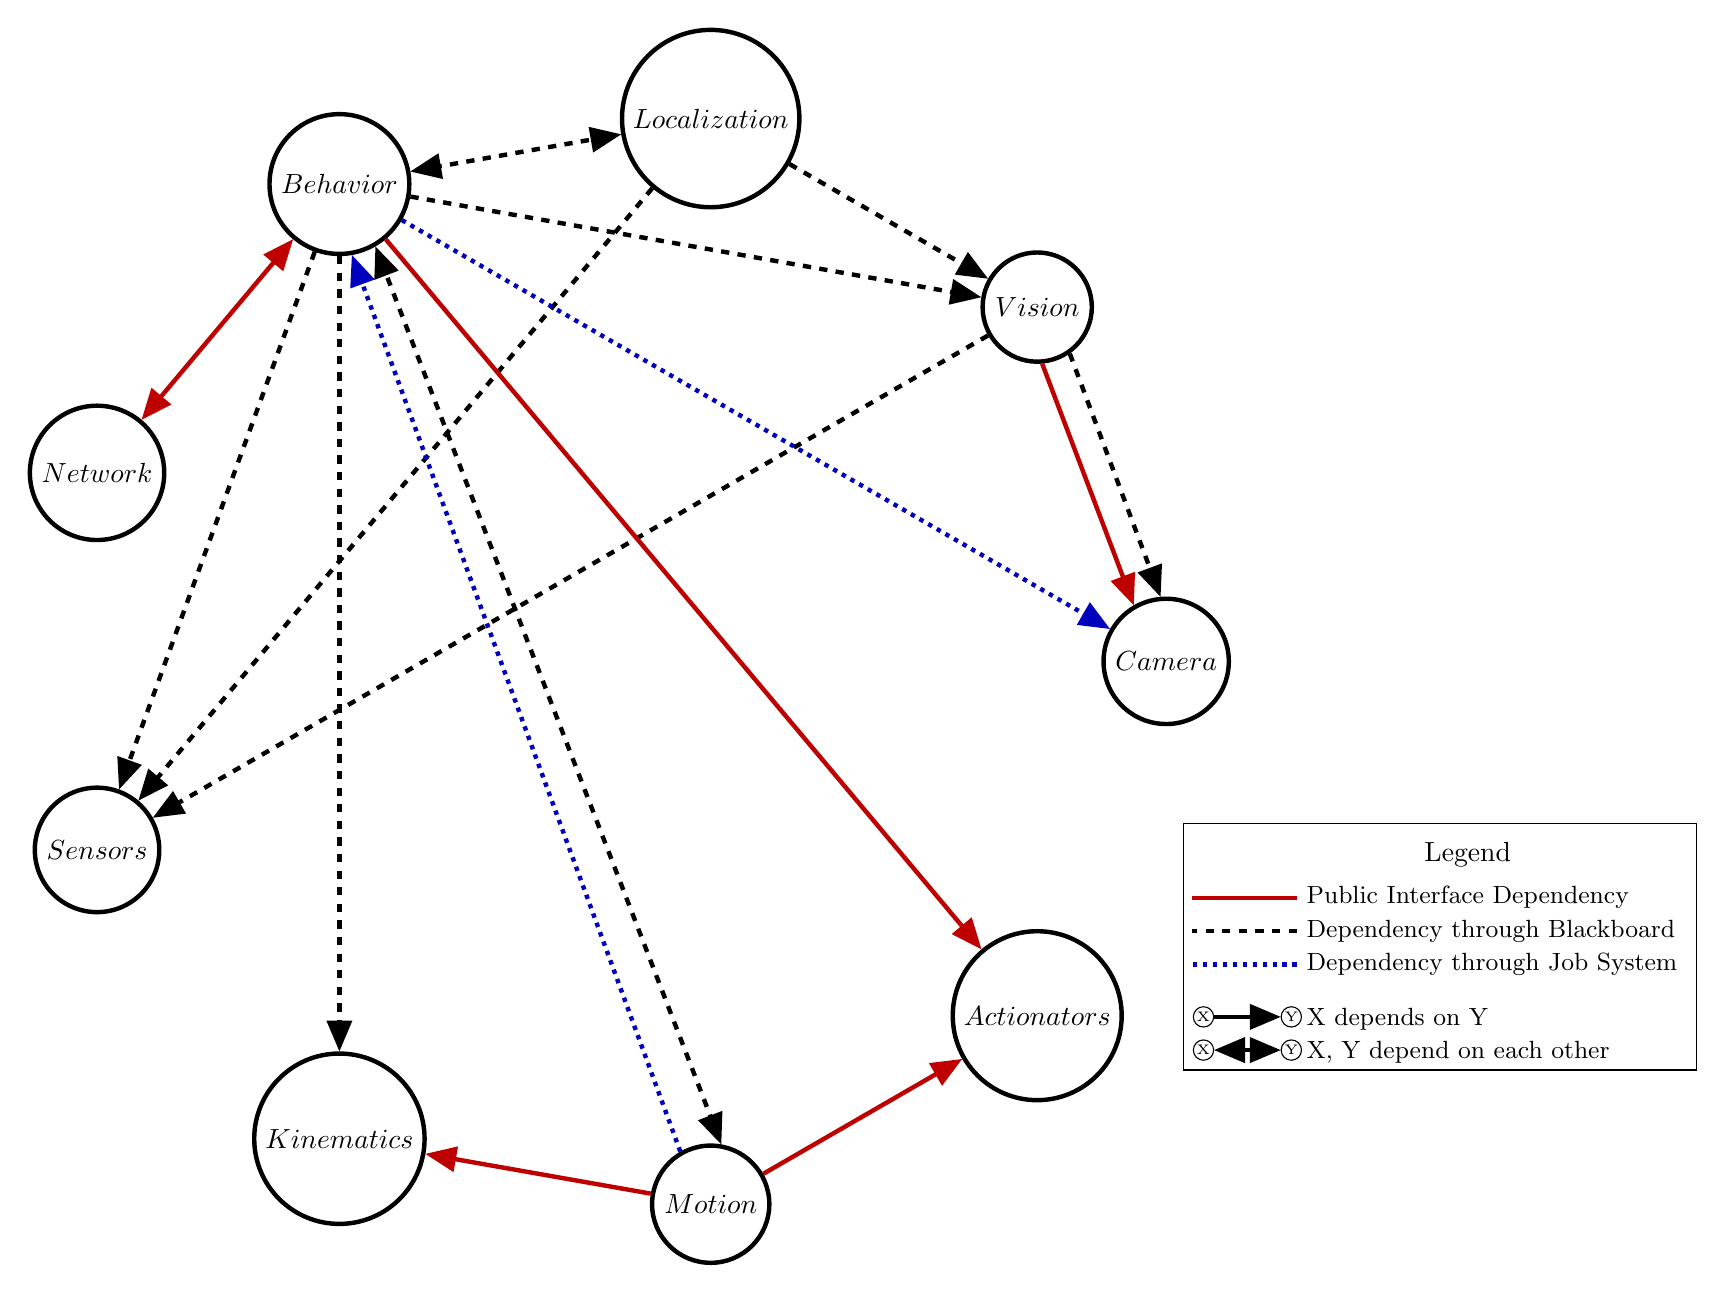
\begin{tikzpicture}[
		reactor/.style={draw, circle, ultra thick}
		, basearrow/.style={>=triangle 45, ultra thick}
		, blackboard/.style={basearrow, dashed}
		, publicinterface/.style={basearrow, color=red!75!black}
		, jobs/.style={basearrow, dotted, color=blue!75!black}
		, dependent/.style={->}
		, codependent/.style={<->}]

		%%% Legend
		\coordinate (legendpoint) at (13, -2);

		%% Public Interface Dependency
		\node [below=of legendpoint,anchor=east] (publicinterfacelabel) {\small Public Interface Dependency};
		\draw [publicinterface] (publicinterfacelabel.mid west) -- ++(-38pt, 0pt);

		%% Blackboard Dependency
		\node [below=12pt of publicinterfacelabel.south west,anchor=south west] (blackboardlabel) {\small Dependency through Blackboard};
		\draw[blackboard] (blackboardlabel.mid west) -- ++(-38pt, 0pt);

		%% Jobs Dependency
		\node [below=12pt of blackboardlabel.south west,anchor=south west] (joblabel) {\small Dependency through Job System};
		\draw[jobs] (joblabel.mid west) -- ++(-38pt, 0pt);

		%% Dependancy Type: Depends on
		\node[below=20pt of joblabel.south west,anchor=south west] (dependencylabel) {\small X depends on Y};
		\node[circle, draw, inner sep=0.5pt] (dependencynodeY) at ([yshift=1pt,xshift=-2pt]dependencylabel.mid west) {\tiny Y};
		\node[circle, draw, inner sep=0.5pt, left=24pt of dependencynodeY] (dependencynodeX) {\tiny X};
		\draw[basearrow, dependent] (dependencynodeX) edge (dependencynodeY);

		%% Dependancy Type: Codependent
		\node[below=12pt of dependencylabel.south west,anchor=south west] (codependencylabel) {\small X, Y depend on each other};
		\node[circle, draw, inner sep=0.5pt] (codependencynodeY) at ([yshift=1pt,xshift=-2pt]codependencylabel.mid west) {\tiny Y};
		\node[circle, draw, inner sep=0.5pt, left=24pt of codependencynodeY] (codependencynodeX) {\tiny X};
		\draw[basearrow, codependent] (codependencynodeX) edge (codependencynodeY);

		%% Legend Header
		\node[above=0pt of publicinterfacelabel] (legendheader) {Legend};

		%%% Draw all of our components in a circle
		\foreach [count=\i] \reactor in {Camera, Vision, Localization, Behavior, Network, Sensors, Kinematics, Motion, Actionators} {
		
			% Draw the reactors around the central star
			\node[reactor] (\reactor) at ({360/9 * (\i - 1)}:7cm) {$\reactor$};
		};

		%% Legend Border
		\node[fit=(legendheader)(publicinterfacelabel)(blackboardlabel)
				(joblabel)(dependencylabel)(codependencynodeX)(codependencynodeY),rectangle,draw](legendgroup){};

		%%% Dependencies
		%% Vision
		\path[blackboard, dependent] (Vision.305) edge (Camera.95);
		\path[publicinterface, dependent] (Vision.275) edge (Camera.120);
		\path[blackboard, dependent] (Vision) edge (Sensors);

		%% Localization
		\path[blackboard, dependent] (Localization) edge (Sensors);
		\path[blackboard, dependent] (Localization) edge (Vision);

		%% Behavior
		\path[blackboard, codependent] (Behavior) edge (Localization);
		\path[blackboard, dependent] (Behavior) edge (Kinematics);
		\path[blackboard, dependent] (Behavior) edge (Vision);
		\path[blackboard, dependent] (Behavior) edge (Sensors);
		\path[publicinterface, dependent] (Behavior) edge (Actionators);
		\path[publicinterface, codependent] (Behavior) edge (Network);
		\path[jobs, dependent] (Behavior) edge (Camera);

		%% Motion
		\path[blackboard, codependent] (Motion.80) edge (Behavior.300);
		\path[jobs, dependent] (Motion.120) edge (Behavior.280);
		\path[publicinterface, dependent] (Motion) edge  (Actionators);
		\path[publicinterface, dependent] (Motion) edge (Kinematics);
	\end{tikzpicture}
	\end{adjustbox}
\end{frame}

\begin{frame}
	\frametitle{Problems in Existing System}
	\begin{itemize}
		\item Hidden Dependencies
			\begin{itemize}
				\item The existing systems dependencies are very poorly defined
				\item For example, localizations dependency on the Stationary/Mobile object system.
				\item These hidden dependencies make it difficult to work on a system without understanding the whole system
			\end{itemize}
	
		\item Threading Issues
			\begin{itemize}
				\item Current system does not handle synchronisation between the two threads well
				\item e.g. The kick system can be prompted mid way by the walk engine, the two can even run together resulting in the robot standing still for prolonged periods.
				\item Happens because the interactions between the two threads is undefined in most cases
			\end{itemize}
	\end{itemize}
\end{frame}

\begin{frame}
	\frametitle{Problems in Existing System}
	\begin{itemize}			
		\item Network Communication
			\begin{itemize}
				\item Network communication is currently entirely through Localisation and Behaviour
				\item Adding new network communication requires modifying these two systems
				\item Because of the difficulty of adding new networking, no new networking will be added
			\end{itemize}
			
		\item Build System
			\begin{itemize}
				\item The current build system uses a make file that calls cmake that builds a make file that is called by the original make file
				\item This makes adding and removing components to the system in a meaningful way difficult
			\end{itemize}
	\end{itemize}
\end{frame}

\begin{frame}
	\frametitle{Wishlist}
	\begin{itemize}
		\item Modular Design
			\begin{itemize}
				\item Many modules that are made for robotics (walk engine, script engine) are useful for more then just soccer.
				\item Being able to use Mock inputs allows the system to be tested without access to a robot
				\item Being able to compose various modules into a binary would allow the robot to do more
				\item Enabling the sharing of these modules between researchers would result in better development (more people using the same code)
			\end{itemize}
			
		\item Transparent Multithreading
			\begin{itemize}
				\item Modern CPUs are getting more cores, rather then becoming faster
				\item Threading is difficult and can almost never be sensibly done at the module level
				\item Threading should be handled by the architecture in a way that can scale up to many cores
			\end{itemize}
	\end{itemize}
\end{frame}
			
\begin{frame}
	\frametitle{Wishlist}
	\begin{itemize}
		\item Runtime Statistics
			\begin{itemize}
				\item When optimising programs for speed it is useful to see how long each section of the code took
				\item Breaking up the modules and timing their execution better shows where CPU time is being used
			\end{itemize}
			
		\item Fine Grained Debugging
			\begin{itemize}
				\item When debugging a large system, there is often a low signal to noise ratio as a lot of debug lines are not useful
				\item Splitting up log lines based on source can help identify problems
				\item Being able to view the call graph in real time on a repeated process helps to identify links
			\end{itemize}
	\end{itemize}
\end{frame}

%----------------------------------------------------------------------------------------
\section{New Design}
%----------------------------------------------------------------------------------------
\begin{frame}
	\sectionpage
\end{frame}

\begin{frame}
	\todo[inline]{Talk about coupling r.e. maintainablity}
	\todo[inline]{Diagram of different forms of coupling}
\end{frame}

\begin{frame}
	\todo[inline]{Describe message passing systems}
	\todo[inline]{How decoupled they are but they need a message passing management system}
\end{frame}

\begin{frame}
	\todo[inline]{Talk about existing systems such as Robot OS, DDX, CORBA}
\end{frame}

\begin{frame}
	\todo[inline]{These are all slow}
\end{frame}

\subsection{NUClear}
\begin{frame}
	\frametitle{NUClear}
	\begin{itemize}
		\item These systems are all too slow to use on a robot
		\item A new system must be designed if message passing is to be used
	\end{itemize}
\end{frame}

\begin{frame}
\begin{itemize}
	\item Problem description
	\item Number of lines of code, estimate of effort
	\item Good Software architecture
	\begin{itemize}
		\item Coupling
		\item Cohesion
	\end{itemize}
	\item Existing system
	\item ROS DDX etc message passing
	\item Metaprogramming
	\item NUClear API
	\begin{itemize}
		\item Message passing
		\item Networking
		\item Multithreading
	\end{itemize}
	\item Benefits
	\begin{itemize}
		\item 
	\end{itemize}
	\item Discuss the ease of adding in things
	\item Robot Dance
	\begin{itemize}
		\item What do they do?
		\item How does it work?
	\end{itemize}
	\item Demonstrate robot dancing
	\item Demonstrate live coding of auto getup script
	\item Demonstrate robot firing missiles
\end{itemize}
\end{frame}

\subsection{NUClear Port}
\begin{frame}
	\frametitle{NUClear Port}

	\begin{itemize}
		\item The NUbots software has been ported to use NUClear
		\item Functionality has been divided into many individual modules
		\item All ommunication across modules is accomplished through NUClear messages
		\item A new, flexible build system has been created with `roles' to allow fast and easy adding of functionality
	\end{itemize}
\end{frame}

\begin{frame}
	\frametitle{Modules}

	\begin{itemize}
		\item Every module has a single clear purpose, for example
		\begin{itemize}
			\item interacting with robot hardware
			\item running scripted movements
			\item loading configuration files
		\end{itemize}
		\item Modules do not care which other modules are present, only what information they consume and what they can produce
		\begin{itemize}
			\item Modules with the same inputs and outputs are interchangeable
			\item Platform details are inherently decoupled from everything else
			\item Only need to understand the modules you're working on, not the entire system
		\end{itemize}
	\end{itemize}
\end{frame}

\begin{frame}
	\frametitle{Modules}

	\todo[inline]{Tikz diagram of the new modules/powerplant model}
\end{frame}

\begin{frame}
	\frametitle{New build system}

	What are roles?
	\begin{itemize}
		\item A group of modules combined to make an executable
		\item We can create new behaviours by combining different modules
		\begin{itemize}
			\item Robocup role with soccer-related modules
			\item Dance role with beat detection and audio input modules
			\item Script Tuner role with an interface for tweaking motion scripts
		\end{itemize}
		\item Only one file needs to be changed to make new roles
		\item Adding new abilities requires very little effort
	\end{itemize}
\end{frame}

\begin{frame}
	\frametitle{Testing}

	\begin{itemize}
		\item Testing is built into the new system from the ground up
		\item Modules have associated unit tests
		\item The build system can run unit tests as a batch
		\item Because of modular design it is easy to test single modules or subsets in isolation
	\end{itemize}
\end{frame}



%----------------------------------------------------------------------------------------
\section{Robot Dance}
%----------------------------------------------------------------------------------------
	\begin{frame}
		\sectionpage %Title page for the Robot Dance section
	\end{frame}
	\subsection{What and Why?} %-------------------
	\begin{frame}
		\frametitle{Robot Dance: What and Why?}
		\begin{itemize}
			\item What does you mean by dancing robots?
			\begin{itemize}
				\item Scripted dancing
				\item Dancing in time with music
			\end{itemize}
			\item Why Dancing Robots?
			\begin{itemize}
				\item Demonstrates the efficiency of the new architecture
				\item Useful for marketing
			\end{itemize}
		\end{itemize}
	\end{frame}
	\subsection{Dancing to Music} %-------------------
	\begin{frame}
		\frametitle{Dancing to Music}
		\begin{itemize}
			\item Music detected through Microphone
			\item Music analysed to find beats
			\item Dance move chosen and scaled to be in time with latest beats
			\item Dance move is enacted
		\end{itemize}
	\end{frame}	
	\subsection{Dancing and NUClear} %-------------------
	\begin{frame}
		\frametitle{Dancing and the New Architecture}
		\framesubtitle{Dancing to a Music}
		\begin{figure}
			\centering
			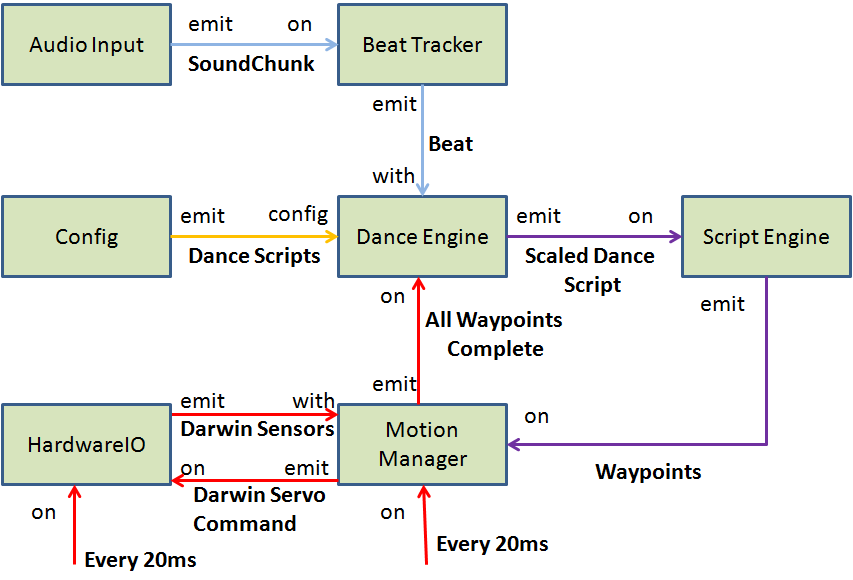
\includegraphics[scale=.45]{Presentation_Images/dance_audio_new_arc.png}
			\caption{Components for Dancing to Music with the NUClear}
		\end{figure}
	\end{frame}	
	\begin{frame}
		\frametitle{Dancing and the New Architecture}
		\framesubtitle{Dancing to a Music}
		\begin{figure}
			\centering
			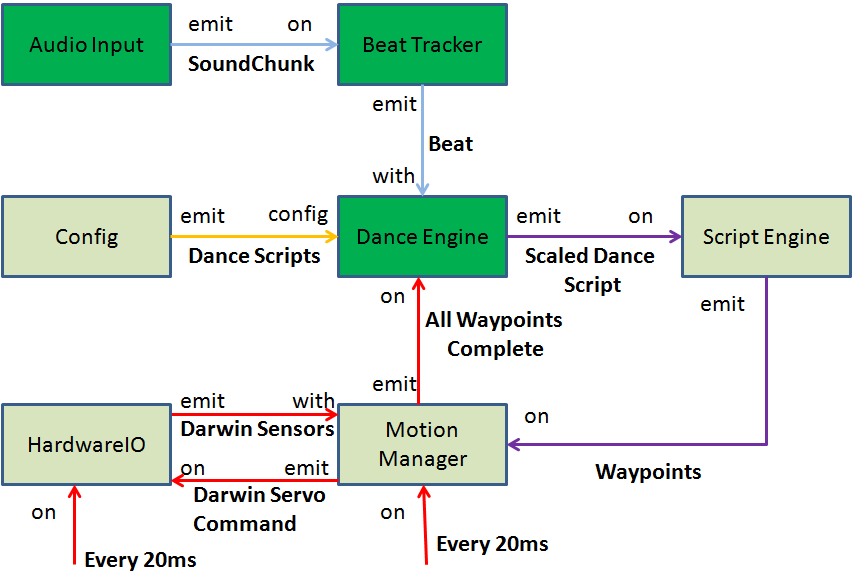
\includegraphics[scale=.45]{Presentation_Images/dance_audio_new_arc_change.png}
			\caption{Components for Dancing to Music with the NUClear}
		\end{figure}
	\end{frame}	
	\subsection{Dancing and the Old Architecture} %-------------------
	\begin{frame} %TODO update this picture
		\frametitle{Dancing and the Old Architecture}
		\framesubtitle{Dancing to a Music}
		\subimport{Presentation_Images/}{dance_audio_old_system.tex}
	\end{frame}	
	\begin{frame} %TODO get rid of this
		\frametitle{Dancing and the Old Architecture}
		\framesubtitle{Dancing to a Music}
		\begin{figure}
			\centering
			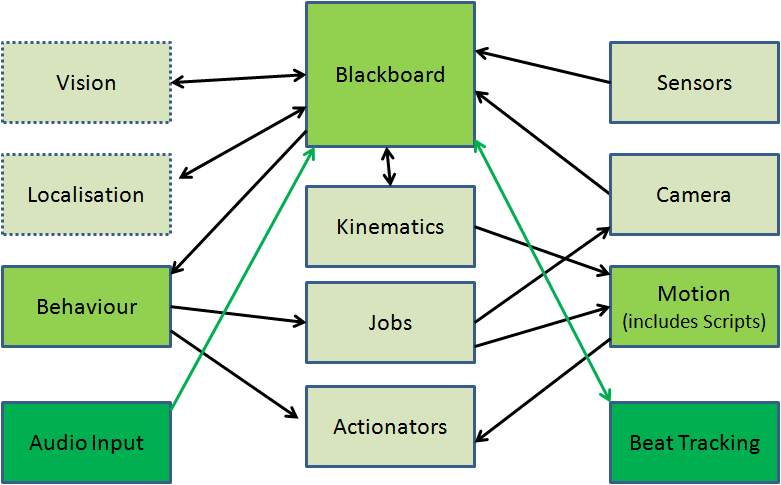
\includegraphics[scale=.45]{Presentation_Images/dance_audio_old_arc.png}
			\caption{Components for Dancing to Music with the Old System}
		\end{figure}
	\end{frame}	
	\subsection{Conclusions} %-------------------
	\begin{frame}
		\frametitle{Conclusions from Robot Dance}
			\begin{itemize}
				\item Robot Dance shows NUClear to be:
				\begin{itemize}
					\item Easy to learn
					\item Easy to use
					\item Modular
					\item Loosely Coupled
				\end{itemize}
			\end{itemize}
	\end{frame}	




%----------------------------------------------------------------------------------------
\section{Individual Research}
%----------------------------------------------------------------------------------------
\begin{frame}
	\sectionpage
\end{frame}

	%----------------------------------------------------------------------------------------
	\subsection{Overcoming Limits of Event Driven Systems}
	%----------------------------------------------------------------------------------------
	\begin{frame}
		\subsectionpage
	\end{frame}
	
	%----------------------------------------------------------------------------------------
	\subsection{Compile Time Message Routing}
	%----------------------------------------------------------------------------------------
	\begin{frame}
		\subsectionpage
	\end{frame}
	
	%----------------------------------------------------------------------------------------
	\subsection{Efficient Multithreading in Message Passing Systems}
	%----------------------------------------------------------------------------------------
	\begin{frame}
		\subsectionpage
	\end{frame}
	
	%----------------------------------------------------------------------------------------
	\subsection{Beat Tracking}
	%----------------------------------------------------------------------------------------
	\begin{frame}
		\subsectionpage
	\end{frame}
	\begin{frame}
		Can Beat Tracking accurately detect beats in real time for Robot Dance?
	\end{frame}
	\begin{frame}
		What is beat tracking?
		\begin{itemize}
			\item Beat is the basic timing element of music
			\item Beats occur at regular intervals
			\item Tapping along to music is beat tracking
			\item Software beat trackers analyse audio input to find the locations of beats.
		\end{itemize}
	\end{frame}
	\begin{frame}
		How a software beat tracker could work
		\begin{itemize}
			\item Onset detection used to find location of musical notes in audio
			\item Notes that occur at regular intervals are found
			\item The most prominent regular notes are taken to be the beat
		\end{itemize}
	\end{frame}
	\begin{frame}
		Criteria for the Beat Tracker:
		\begin{itemize}
			\item Real Time % Whole piece of music doesn't need to be analysed. Works with microphone input.
			\item Quick % Doesn't slow down other systems. Beat found before the next beat occurs.
			\item Accurate % Beats found are close enough to where a listener feels they should be
			\item Robust	% Works in real audio situations with background noise an Robot motor noise.		
		\end{itemize}
	\end{frame}
	\begin{frame}
		Real Time:
		\begin{itemize}
			\item Does not require analysing the whole song to find the beats
			\item Uses past events to find beats but not future events.
			\item Can take in audio through microphone and analyse incrementally
		\end{itemize}		
	\end{frame}
	\begin{frame}
		Quick:
		\begin{itemize}
			\item Doesn't slow down the rest of the system.
			\item Beat located before next audio containing a beat is input into system
		\end{itemize}		
	\end{frame}
	\begin{frame}
		Accurate:
		\begin{itemize}
			\item Measures highly on beat tracker evaluation tests
			\item Beats found feel right to a listener.
			\item Accuracy doesn't need to be perfect
			\begin{itemize}
				\item Can't be perfectly on the beat
				\item Half-pace beats may still feel right to a user
			\end{itemize}	
		\end{itemize}		
	\end{frame}
	\begin{frame}
		Robust:
		\begin{itemize}
			\item Works in real audio situations
			\item Able to ignore background noise
			\item Biggest problem for robots is motor noise
		\end{itemize}		
	\end{frame}
	\begin{frame}
		Two Candidates:
		\begin{itemize}
			\item Aubio
				\begin{itemize}
					\item Not the most accurate but it is quick
				\end{itemize}
			\item Beat'n
				\begin{itemize}
					\item Beat tracker Trent wrote when we were trying to get Aubio to work
				\end{itemize}
		\end{itemize}		
	\end{frame}
	\begin{frame}
		Testing the 2 Beat Trackers for accuracy:
		\begin{itemize}
			\item Tested on 20, thirty second snippets of music
			\item Compared results of Beat Trackers with beats found by a human
			\item Comparisons evaluated by 6 evaluation methods (some with several variations)
			\item In addition to testing Aubio and Beat'n, we also test a dummy algorithm which simply has a beat occur every 0.5 seconds
		\end{itemize}		
	\end{frame}
%	\begin{frame}
%		Testing results:
%		\begin{table}
%		\begin{tabular}{c c c c c c c c c c c}
%			          & F-Measure & Cem(acc) & Goto(acc) & P-Score & CMLc & CMLt & AMLc & AMLt & D & Dg \\
%			Aubio & 29.6205 & 20.9227 & 0 & 35.5261 & 9.3504 & 14.2556 & 20.0702 & 31.6623 & 0.9857 & 0.0723 \\
%			Beat'n & 22.8261 & 15.7258 & 0 & 28.6636 & 3.054 & 5.8672 & 17.6479 & 25.7328 & 0.9178 & 0.0527 \\
%			Dummy & 8.227 & 5.7759 & 0 & 7.0067 & 0.7358 & 1.6722 & 1.5552 & 3.3445 & 0.0253 & 0.0083 \\
%		\end{tabular}
%		\end{table}	
%	\end{frame}
	\begin{frame}
		Testing results:
		\begin{table}
		\begin{tabular}{c | c | c | c }
			  & Aubio  & Beat'n  & Dummy\\ \hline
			F-Measure  & 29.62  & 22.83  & 27.93\\ \cline{1-1}  \cdashline{2-4}
			Cem(acc)  & 20.92  & 15.73  & 19.61\\ \cline{1-1}  \cdashline{2-4}
			Goto(acc)  & 0  & 0  & 0\\ \cline{1-1}  \cdashline{2-4}
			P-Score  & 35.53  & 28.66  & 36.91\\ \cline{1-1}  \cdashline{2-4}
			CMLc  & 9.35  & 3.05  & 4.16\\ \cline{1-1}  \cdashline{2-4}
			CMLt  & 14.26  & 5.87  & 9.37\\ \cline{1-1}  \cdashline{2-4}
			AMLc  & 20.07  & 17.65  & 8.87\\ \cline{1-1}  \cdashline{2-4}
			AMLt  & 31.66  & 25.73  & 19.07\\ \cline{1-1}  \cdashline{2-4}
			D  & 0.99  & 0.92  & 0.59\\ \cline{1-1}  \cdashline{2-4}
			Dg  & 0.0723  & 0.0527  & 0.0315\\ \cline{1-1}  \cdashline{2-4}
		\end{tabular}
		\end{table}	
	\end{frame}
	\begin{frame}
		Further testing for Aubio:
		\begin{itemize}
			\item Tested on 14 songs
			\item Compared with more modern beat trackers
		\end{itemize}		
	\end{frame}
	\begin{frame}
		Testing results:
		\begin{table}
		\begin{tabular}{c | c | c | c | c | c | c}
			& Davies & Kea & Dixon & Ellis & Dummy & Aubio \\ \hline
			F-Measure & 82.16 & 87.56 & 91.93 & 79.78 & 27.65 & 25.36 \\ \cline{1-1}  \cdashline{2-7}
			Cem(acc)  & 80.75 & 73.72 & 86.14 & 52.08 & 19.41 & 18.42 \\ \cline{1-1}  \cdashline{2-7}
			Goto(acc)  & 100 & 78.57 & 85.71 & 35.71 & 0 & 7.14 \\ \cline{1-1}  \cdashline{2-7}
			P-Score &  79.94 & 82.49 & 90.29 & 72.07 & 35.38 & 35.05 \\ \cline{1-1}  \cdashline{2-7}
			CMLc  & 76.45 & 58.68 & 76.62 & 37.17 & 4.54 & 7.82 \\ \cline{1-1}  \cdashline{2-7}
			CMLt  & 77.94 & 68.82 & 84.04 & 48.2 & 18.63 & 21.51 \\ \cline{1-1}  \cdashline{2-7}
			AMLc  & 77.26 & 79.95 & 79.84 & 39.72 & 4.93 & 16.12 \\ \cline{1-1}  \cdashline{2-7}
			AMLt  & 78.72 & 90.09 & 90.98 & 77.58 & 19.81 & 36.75 \\ \cline{1-1}  \cdashline{2-7}
			D  & 3.28 & 2.4 & 2.74 & 2.64 & 0.095 & 0.45 \\ \cline{1-1}  \cdashline{2-7}
			Dg  & 2.85 & 1.85 & 2.36 & 1.63 & 0.013 & 0.023 \\ \cline{1-1}  \cdashline{2-7}
		\end{tabular}
		\end{table}	
	\end{frame}
	\begin{frame}
		Difficulties with testing:
		\begin{itemize}
			\item Acquiring music with annotated beat locations
			\item Offbeats counted as completely wrong
			\item Dummy algorithm can score high, but conveys no information
		\end{itemize}
	\end{frame}
	\begin{frame}
		Evaluating the other criteria:
		\begin{itemize}
			\item Both algorithms work in real time
			\item Both algorithms are quick
			\item Aubio has big problems with Motor Noise, though a filter could fix it.
			\item Beat'n handle motor noise much better, though it still has some problem with it
		\end{itemize}
	\end{frame}
	\begin{frame}
		Conclusion:
		\begin{itemize}
			\item Beat Tracking CAN accurately detect beats in real time for Robot Dance
			\item Aubio and Beat'n are a little lacking but sufficient for the job
			\item Better beat trackers are available, particuarly when more processing power is available.
		\end{itemize}
	\end{frame}
	\begin{frame}
		Core Papers:
		
	\end{frame}
	
\end{document} 
